\documentclass[11pt, oneside]{article} 
\usepackage{geometry}
\geometry{letterpaper} 
\usepackage{graphicx}
	
\usepackage{amssymb}
\usepackage{amsmath}
\usepackage{parskip}
\usepackage{color}
\usepackage{hyperref}

\graphicspath{{/Users/telliott_admin/Dropbox/Tex/png/}}
% \begin{center} 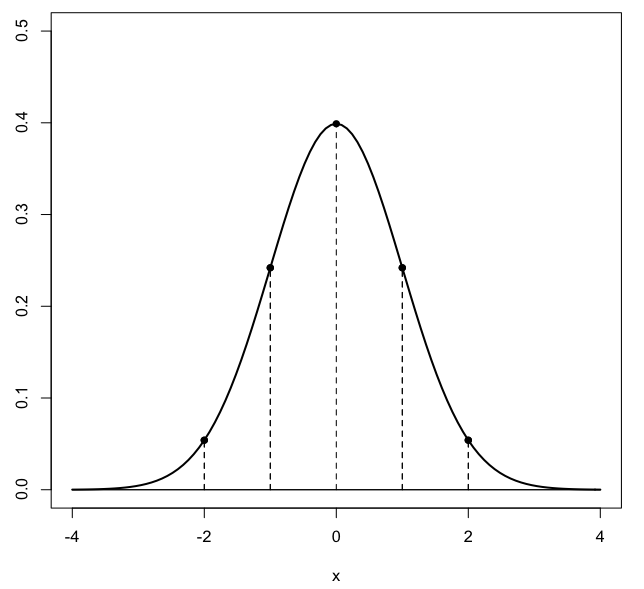
\includegraphics [scale=0.4] {gauss3.png} \end{center}

\title{Pythagoras}
\date{}

\begin{document}
\maketitle
\Large

The most famous theorem of Greek geometry is also the most useful in Calculus.  
\begin{center} 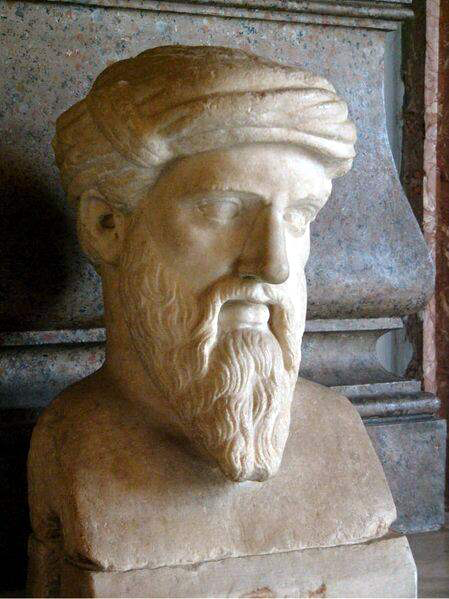
\includegraphics [scale=0.3] {pythagoras.png} \end{center}

Here are some proofs.  First a visual one:
\begin{center} 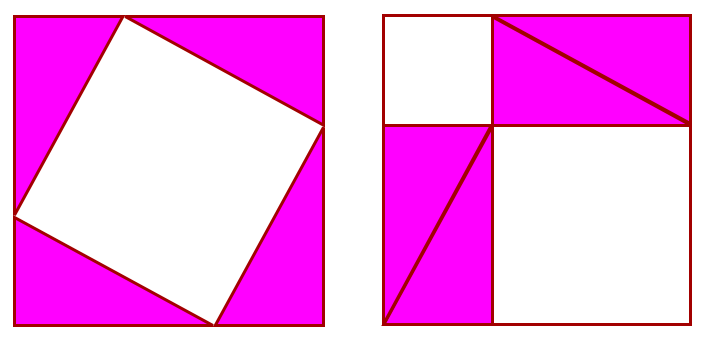
\includegraphics [scale=0.4] {pythagoras1.png} \end{center}

It really needs no explanation, but ..

In the left panel we have a large square box that contains a white square whose side is also the hypotenuse of the four identical right triangles contained inside.  Altogether the four triangles plus the white area adds up to the total.

We simply rearrange the triangles.  Now we evidently have the same area left over from the four triangles, because they still have the same area and the box has not changed.  

But clearly, now the white area is the sum of the squares on the second and third sides of the triangles.  Hence the two white squares on the right are equal in area to the large white square on the left.

The second proof relies on the following construction (Euclid $I.47$, sometimes called the "bridal chair"), where the central triangle is a right triangle, and the other constructions are squares.

\begin{center} 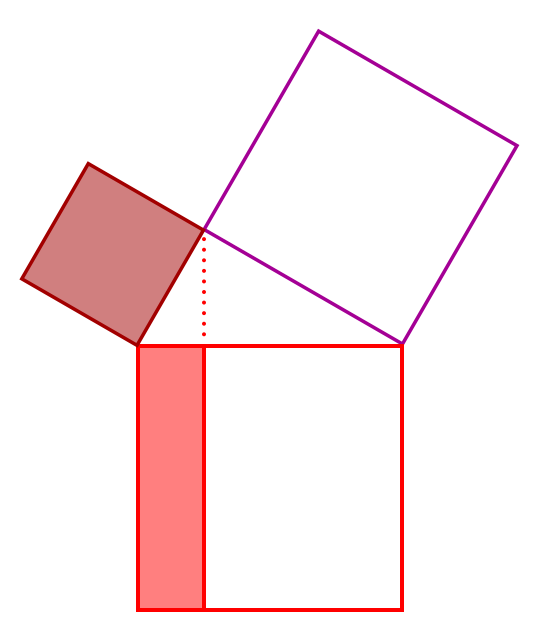
\includegraphics [scale=0.35] {pythagoras2.png} \end{center}

What we will show is that the part of the large square in red is equal in area to the entire small square, in maroon.

We label some points as shown:
\begin{center} 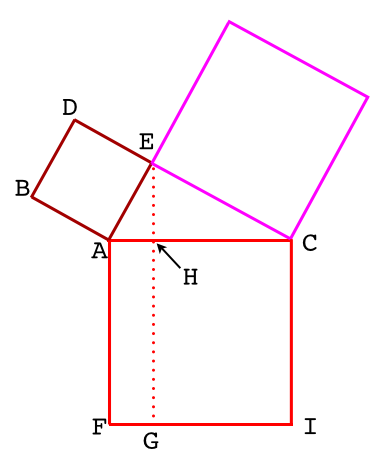
\includegraphics [scale=0.45] {pythagoras3.png} \end{center}
   
We drop a vertical line $EHG$, constructing the rectangle $AFGH$.
   
Finally we sketch dotted lines for the long sides of two triangles:
\begin{center} 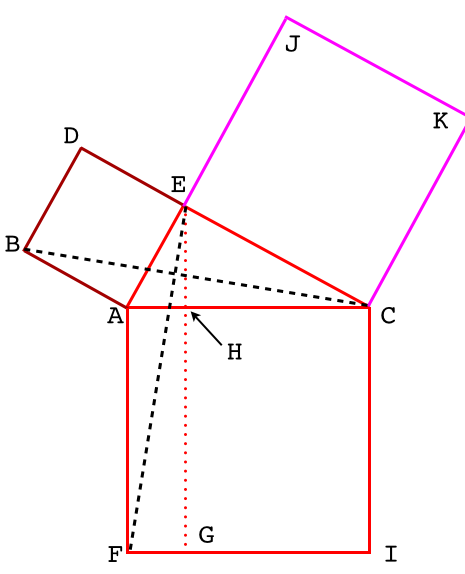
\includegraphics [scale=0.4] {pythagoras4.png} \end{center}

Triangle $\Delta ABC$ is congruent to triangle $\Delta AEF$.  

We use "side-angle-side".  The two sets of sides are evidently equal 
\[ AB = AE \]
\[ AC = AF \]

What about the included angle?  Both angle $\angle BAC$ and $\angle EAF$ contain right angles plus a shared angle in the middle, $\angle EAC$.  So they are themselves equal, and thus we have proved the congruence relationship:
\[ \Delta ABC = \Delta AEF \]

The next part of the proof is to see that triangle $\Delta ABC$ has base $AB$ and altitude $AE$ so its area is half that of the small square $ABDE$.  On the other hand triangle $\Delta AEF$ has base $AF$ and altitude $AH$ (as well as $FG$) so its area is half that of the rectangle $AFGH$.

Hence we have proved that the two colored areas in this figure are equal:

\begin{center} 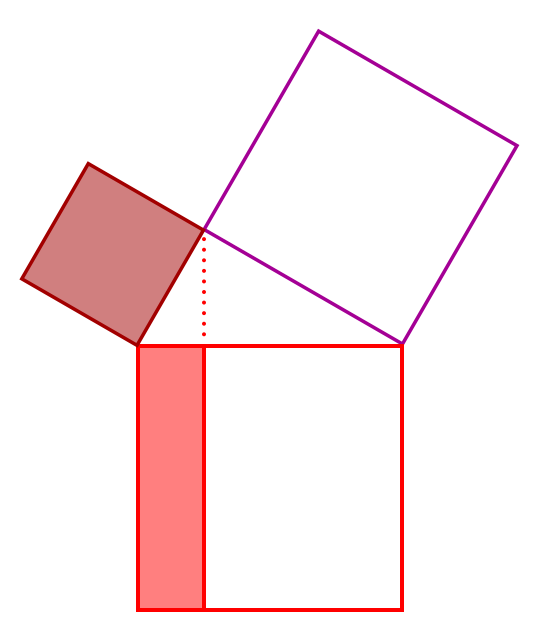
\includegraphics [scale=0.35] {pythagoras2.png} \end{center}
Finally, we could proceed to do the same thing on the right side of the figure, but we just appeal to symmetry.  All the equivalent relationships will hold.

The third proof is an algebraic one.  Not so pretty, but it is fast.  We divide a right triangle into two smaller ones by dropping an altitude.
\begin{center} 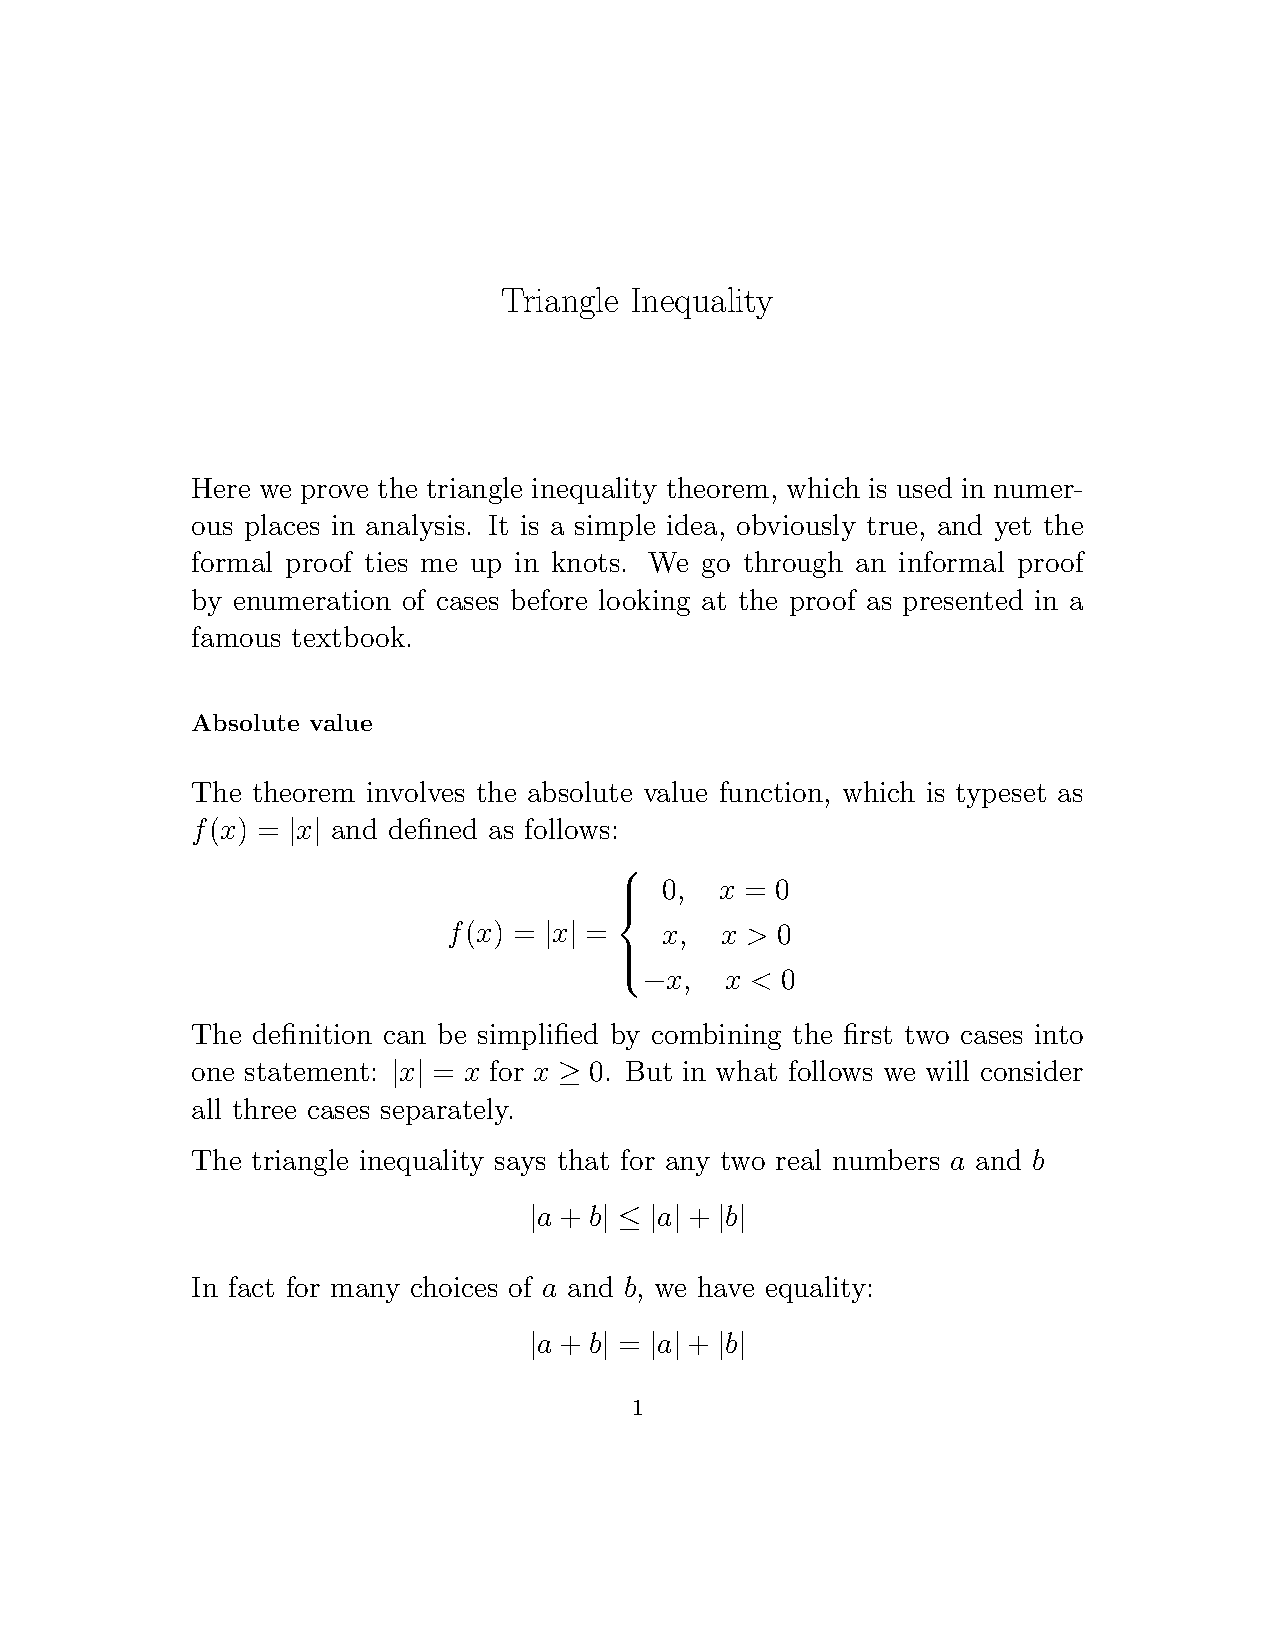
\includegraphics [scale=0.5] {triangle.png} \end{center}

By complementary angles, these three triangles are all similar (e.g., the angle between sides $b$ and $h$ is equal to that between sides $a$ and $c$).  So we can construct ratios of sides that are equal.

We need a relationship involving $a^2$.  We look for one involving $c$ and $e$:
\[ \frac{e}{a} = \frac{a}{c} \]
\[ a^2 = ce \]
\begin{center} 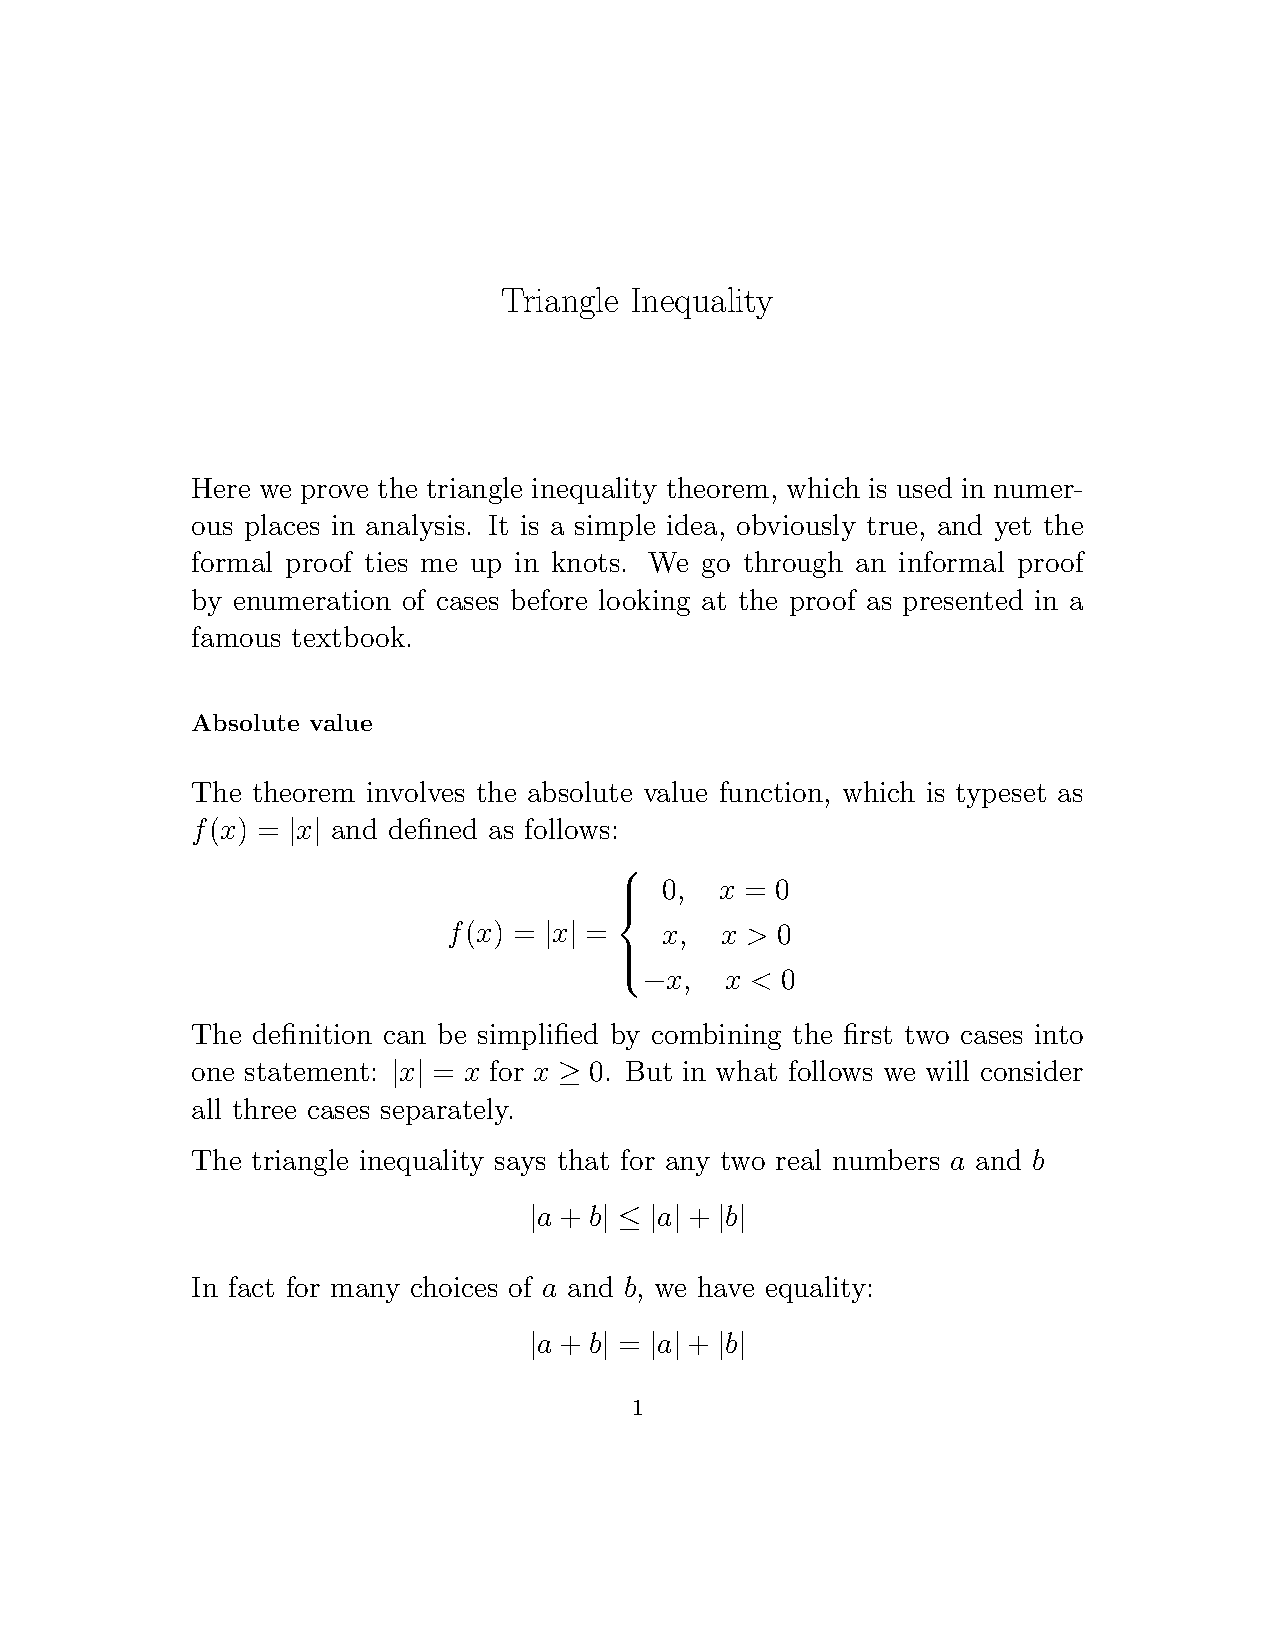
\includegraphics [scale=0.5] {triangle.png} \end{center}

and a relationship between $b^2$ and $c^2$:

\[  \frac{b}{d} = \frac{c}{b}  \]
\[  b^2 = cd  \]

Putting the two together:
\[ a^2 + b^2 = ce + cd \]
\[ = c (d+e) = c^2 \]

Which is what we wanted to prove.

There are more than 300 proofs of this theorem, including one by a President of the United States.

\end{document}